\documentclass{article}
\usepackage[utf8]{inputenc}
\usepackage{graphicx}
\usepackage{geometry}
\usepackage{listings}
\usepackage{hyperref}

\geometry{
 a4paper,
 total={170mm,257mm},
 left=20mm,
 top=20mm,
}

\title{Pr\'actica 5: Aplicaci\'on de Gesti\'on de Tareas con Navegaci\'on y Carga Diferida}
\author{Kirbi Xavier Huerta Salinas}
\date{Octubre 2025}

\begin{document}

\maketitle

\section{Introducci\'on}
El presente documento detalla el desarrollo de una aplicaci\'on m\'ovil para la gesti\'on de tareas, construida con Ionic y Angular. El objetivo de la pr\'actica es aplicar conceptos clave de desarrollo de aplicaciones m\'oviles, como la creaci\'on de componentes, navegaci\'on, persistencia de datos y optimizaci\'on de carga.

La aplicaci\'on permite a los usuarios crear, visualizar, editar y eliminar tareas, las cuales se almacenan localmente en el dispositivo para garantizar la persistencia de la informaci\'on entre sesiones.

\section{Cumplimiento de Requisitos}
La aplicaci\'on implementa todos los requisitos solicitados en el documento de la pr\'actica:
\begin{itemize}
    \item \textbf{Creaci\'on de P\'aginas:} Se crearon tres p\'aginas principales: \texttt{Home} (para listar tareas), \texttt{Tarea} (para crear una nueva tarea) y \texttt{TareaDetalles} (para editar una tarea existente).
    \item \textbf{Navegaci\'on:} Se configur\'o un sistema de rutas en Angular para navegar entre las p\'aginas mencionadas.
    \item \textbf{Lazy Loading:} Todas las rutas de las p\'aginas se implementaron con carga diferida (lazy loading) utilizando la funci\'on \texttt{loadComponent} para optimizar el rendimiento inicial de la aplicaci\'on.
    \item \textbf{Servicio y Persistencia:} Se desarroll\'o un servicio (\texttt{TareaService}) que centraliza la l\'ogica de negocio (CRUD) y utiliza el \texttt{localStorage} del navegador para guardar y recuperar las tareas.
    \item \textbf{Dise\~no de UI:} La interfaz es sencilla y funcional, utilizando los componentes de Ionic para una experiencia de usuario nativa.
    \item \textbf{Validaciones:} El formulario de creaci\'on y edici\'on de tareas incluye validaciones para campos requeridos y para asegurar que la fecha de vencimiento sea siempre una fecha futura.
\end{itemize}

\section{Estructura y Organizaci\'on del Proyecto}
El proyecto sigue la estructura est\'andar de una aplicaci\'on de Angular, con los componentes de la aplicaci\'on ubicados en la carpeta \texttt{src/app}. Las p\'aginas, servicios y modelos de datos se organizaron en sus respectivas carpetas para mantener el c\'odigo ordenado y mantenible.

\begin{itemize}
    \item \texttt{src/app/pages/}: Contiene los componentes de p\'agina (\texttt{TareaPage}, \texttt{TareaDetallesPage}).
    \item \texttt{src/app/services/}: Contiene el servicio de l\'ogica de negocio (\texttt{TareaService}).
    \item \texttt{src/app/models/}: Define la interfaz del modelo de datos (\texttt{Tarea}).
    \item \texttt{src/app/validators/}: Contiene validadores de formularios personalizados.
\end{itemize}

\section{Detalles de Implementaci\'on}

\subsection{Uso de Lazy Loading}
La carga diferida se configur\'o en \texttt{src/app/app.routes.ts}. Cada ruta utiliza \texttt{loadComponent} para cargar los componentes de p\'agina solo cuando son necesarios.

\begin{lstlisting}[breaklines=true]
import { Routes } from '@angular/router';

export const routes: Routes = [
  {
    path: 'home',
    loadComponent: () => import('./home/home.page').then((m) => m.HomePage),
  },
  {
    path: 'tarea',
    loadComponent: () => import('./pages/tarea/tarea.page').then( m => m.TareaPage)
  },
  {
    path: 'tarea-detalles/:id',
    loadComponent: () => import('./pages/tarea-detalles/tarea-detalles.page').then( m => m.TareaDetallesPage)
  },
];
\end{lstlisting}

\subsection{Persistencia con LocalStorage}
El servicio \texttt{TareaService} es responsable de interactuar con \texttt{localStorage} para persistir los datos. Los m\'etodos \texttt{saveTareas} y \texttt{getTareas} se encargan de la serializaci\'on y deserializaci\'on de los datos de las tareas.

\begin{lstlisting}[breaklines=true]
@Injectable({
  providedIn: 'root'
})
export class TareaService {
  private readonly storageKey = 'tareas';

  getTareas(): Tarea[] {
    const tareasJson = localStorage.getItem(this.storageKey);
    if (tareasJson) {
      return JSON.parse(tareasJson).map((tarea: any) => ({
        ...tarea,
        fechaVencimiento: new Date(tarea.fechaVencimiento)
      }));
    }
    return [];
  }

  private saveTareas(tareas: Tarea[]): void {
    localStorage.setItem(this.storageKey, JSON.stringify(tareas));
  }
  // ... otros metodos CRUD
}
\end{lstlisting}

\subsection{Validaciones de Formulario}
Se utiliz\'o un validador personalizado (\texttt{fechaFuturaValidator}) para el campo de fecha, asegurando que el usuario no pueda seleccionar una fecha que ya ha pasado. Este validador se combina con los validadores est\'andar de Angular para campos requeridos.

\begin{lstlisting}[breaklines=true]
// En el componente TareaPage o TareaDetallesPage
this.tareaForm = this.fb.group({
  titulo: ['', Validators.required],
  descripcion: ['', Validators.required],
  fechaVencimiento: [null, [Validators.required, fechaFuturaValidator]]
});

// Mensaje de error en el HTML
<div *ngIf="tareaForm.get('fechaVencimiento')?.hasError('fechaPasada')">
  La fecha debe ser futura.
</div>
\end{lstlisting}

\section{Capturas de Pantalla}

\begin{figure}[htbp]
\centering
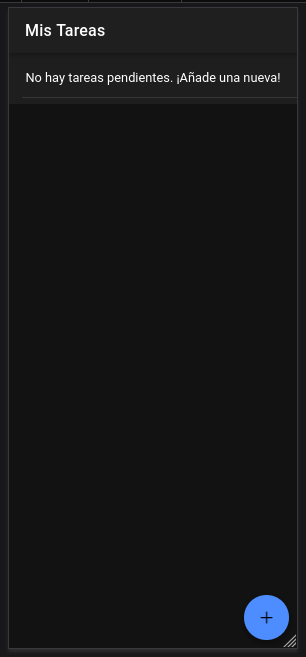
\includegraphics[width=0.4\textwidth]{captura_home.png}
\caption{P\'agina principal con la lista de tareas.}
\label{fig:home}
\end{figure}
\begin{figure}[htbp]
\centering

\includegraphics[width=0.4\textwidth]{captura_crear.png}
\caption{Formulario de creaci\'on de una nueva tarea.}
\label{fig:crear}
\end{figure}
\begin{figure}[htbp]
\centering
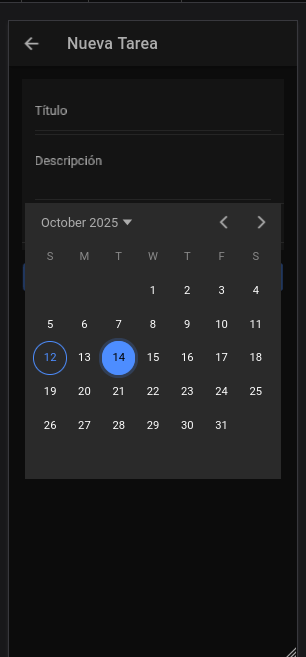
\includegraphics[width=0.4\textwidth]{captura_fecha.png}
\caption{ion-datetime para seleccionar la fecha de vencimiento.}
\label{fig:datetime}
\end{figure}
\begin{figure}[htbp]
\centering
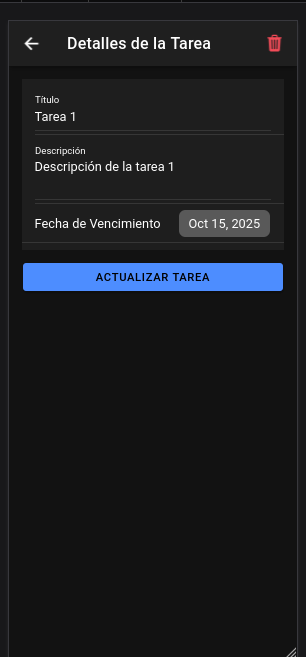
\includegraphics[width=0.4\textwidth]{captura_detalles.png}
\caption{Formulario de edici\'on de una tarea existente.}
\label{fig:detalles}
\end{figure}
\begin{figure}[htbp]
\centering
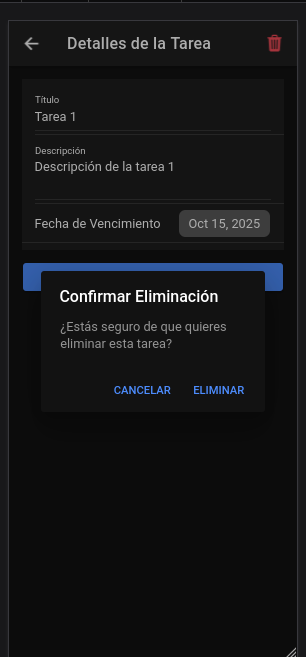
\includegraphics[width=0.4\textwidth]{captura_eliminar.png}
\caption{Mensaje al querer eliminar una tarea.}
\label{fig:eliminar}
\end{figure}


\section{Compilaci\'on para Android con Capacitor}
Para empaquetar la aplicaci\'on para Android, se utiliz\'o Capacitor. Este proceso convierte la aplicaci\'on web en un proyecto nativo de Android que puede ser gestionado con Android Studio.

Los pasos seguidos fueron los siguientes:
\begin{enumerate}
    \item \textbf{Instalar dependencias de Capacitor:}
    \begin{verbatim}
npm install @capacitor/core @capacitor/cli
    \end{verbatim}

    \item \textbf{Inicializar Capacitor:} Se crea el archivo de configuraci\'on principal.
    \begin{verbatim}
npx cap init
    \end{verbatim}

    \item \textbf{Construir la aplicaci\'on web:} Se generan los archivos est\'aticos del proyecto de Angular.
    \begin{verbatim}
npm run build
    \end{verbatim}

    \item \textbf{A\~nadir la plataforma Android:} Se crea el proyecto nativo de Android.
    \begin{verbatim}
npx cap add android
    \end{verbatim}

    \item \textbf{Sincronizar los recursos web:} Se copian los archivos web al proyecto nativo.
    \begin{verbatim}
npx cap sync
    \end{verbatim}

    \item \textbf{Abrir en Android Studio:} Finalmente, se abre el proyecto en el IDE de Android para compilar y ejecutar.
    \begin{verbatim}
npx cap open android
    \end{verbatim}
\end{enumerate}

\section{Demostraci\'on en Video}
Se grab\'o un video que muestra la aplicaci\'on funcionando en un dispositivo m\'ovil Android. El video demuestra la creaci\'on, edici\'on, y eliminaci\'on de tareas, as\'i como la correcta funcionalidad de las validaciones y la persistencia de datos.

El video se puede visualizar en el siguiente enlace:
\href{https://correobuap-my.sharepoint.com/:v:/g/personal/kirbi_huertas_alumno_buap_mx/ERhO-CAdlztNmy3Wuwh2q4IB6dL--OChuUR7Iv7fA9dB9Q?nav=eyJyZWZlcnJhbEluZm8iOnsicmVmZXJyYWxBcHAiOiJPbmVEcml2ZUZvckJ1c2luZXNzIiwicmVmZXJyYWxBcHBQbGF0Zm9ybSI6IldlYiIsInJlZmVycmFsTW9kZSI6InZpZXciLCJyZWZlcnJhbFZpZXciOiJNeUZpbGVzTGlua0NvcHkifX0&e=i78Fpx}{Ver video de la aplicación en funcionamiento}


\end{document}
